% siminos/CLE/symDyn.tex
% $Author$ $Date$

% symmetry in dynamical systems

Consider a system of \ode s of the form
\beq
	\dot{\ssp} = \vf(\ssp)
	\label{eq:difeq}
\eeq
where $\vf: \pS \rightarrow \pS$ a $C^\infty$ mapping and $\pS\subset\Rls{n}$
a manifold. Any compact Lie group acting on $\Rls{n}$ can be identified
with a subgroup of $\On{n}$, \cf\ for example \refref{golubII},
so we concentrate on subgroups $\Group\subseteq\On{n}$ in what
follows, following, without loss of generality.
%
%\ES{Can we generalize this to say that any compact Lie group acting on a
%manifold can be can be identified with a subgroup of $\On{n}$ acting on $\Rls{n}$?}
% PC: OK
Here the emphasis is on continuous symmetry, so we will
restrict attention to compact Lie groups. Though the example studied here
will involve a one parameter \SOn{2},
generalization to higher-dimensional Lie groups is immediate.

A group element $\LieEl\in\On{n}$ is a symmetry of
\refeq{eq:difeq} if for every solution $x(t)$, $\LieEl x(t)$ is
also a solution. Equivalently, $\LieEl$ is a symmetry of
\refeq{eq:difeq} if 
\beq
	\vf(\LieEl x) =\LieEl \vf(x)
	\label{eq:equiv} 
\eeq 
for all $x\in\Rls{n}$. We say that
$\vf$ \emph{commutes} with $\LieEl$ or that $\vf$ is
$\LieEl$-\emph{equivariant}. When $\vf$ commutes with all
$\LieEl\in\Group$ we say that $\vf$ is $\Group$-equivariant.
The finite time flow $\flow{t}{\LieEl x_o}$ through $\LieEl
x_o$ satisfies the equivariance condition
\beq\label{eq:equivFinite} 
\flow{t}{\LieEl x_o}=\LieEl\flow{t}{x_o} 
\eeq 
from definition of symmetry and
uniqueness of solutions. In physics literature the term
$invariant$ is most commonly used; in
Hamiltonian systems a symmetry is manifested as invariance of the
Hamiltonian under the symmetry group action.
%\ES{To Predrag: Do you agree with this statement?}.
% PC: OK


An element of a compact Lie group
continuously connected to identity can be written as
\beq
\LieEl(\gSpace)=e^{\gSpace \cdot \Lg }
	\,,\qquad
\gSpace \cdot \Lg  = \sum \gSpace_a \Lg_a,\; a=1,2, \cdots, N
\,,
\ee{FiniteRot}
where
$\gSpace \cdot \Lg$
is a {\em Lie algebra} element,  and $\gSpace_a$ are the parameters
of the transformation.
{Unitary} transformations $ \exp(\gSpace \cdot {\Lg}) $ are
generated by sequences of infinitesimal steps of form
\beq
\LieEl(\delta\gSpace) \simeq 1 + \delta \gSpace \cdot \Lg
% \LieEl{}_i{}^j \simeq \delta_i^j +  \delta \gSpace_a \, (\Lg_a)_i^j
    \,,\quad
\delta\gSpace \in \reals^N
    \,,\quad
|\delta \gSpace| \ll 1
    \, ,
\ee{intsmLieTransf}
where $\Lg_a$, the {\em generators} of infinitesimal
transformations, are a set of linearly independent
$[d\!\times\!d]$ anti-hermitian matrices, $(\Lg_a)^\dagger =
- \Lg_a$, acting linearly on the $d$-dim\-ens\-ion\-al \statesp\
$\pS$. Repeated indices are summed throughout this section.

For continuous groups the {Lie algebra}, \ie,
the set of $N$ generators $\Lg_a$ of infinitesimal
transformations, takes the role that the $|\Group|$ group
elements play in the theory of discrete groups. The flow field
at the \statesp\ point $\ssp$ induced by the action of the group
is given by the set of $N$ tangent fields
\beq
\groupTan_a(\ssp)_{i}= (\Lg_a){}_{i}{}^j \ssp_j
\,.
\ee{GroupTangField}

% \example{Finite angle \SOn{2} rotations:}{
% \label{exam:FinRot}
% Substituting the Lie algebra generator
%     \PC{is the sign standard?}
% \beq
%  \Lg \,=\,   \left(\barr{ccccc}
%     0  &  1 & 0  &  0 & 0  \\
%    -1  &  0 & 0  &  0 & 0 \\
%     0  &  0 & 0  &  1 & 0  \\
%     0  &  0 &-1  &  0 & 0 \\
%     0  &  0 & 0  &  0 & 0
%     \earr\right)
% \ee{CLfLieGen}
% acting on a 5-dim\-ens\-ion\-al space into \refeq{FiniteRot} yields
% a finite angle \SOn{2} rotation:
% \beq
% \LieEl(\gSpace) \,=\,  \left(\barr{ccccc}
%   \cos \gSpace  & \sin \gSpace  & 0 & 0 & 0 \\
%  -\sin \gSpace  & \cos \gSpace  & 0 & 0 & 0 \\
%  0 & 0 &  \cos \gSpace & \sin \gSpace   & 0 \\
%  0 & 0 & -\sin \gSpace & \cos \gSpace   & 0 \\
%  0 & 0 & 0             & 0              & 1
%     \earr\right)
% \,.
% \ee{CLfRots}
% The generator $\Lg$ is indeed anti-hermitian,
% $\Lg^\dagger = - \Lg$, and the group is compact, its
% elements parametrized by $\gSpace \mbox{ mod } 2\pi$. Locally, at
% $\ssp \in \pS$, the infinitesimal action of the group is
% given by the group tangent field $\groupTan(\ssp) = \Lg \ssp
% = (x_2,-x_1,y_2,-y_1,0)$. In other words, the flow induced by
% the group action is normal to the radial direction in the
% $(x_1,x_2)$ and $(y_1,y_2)$ planes, while the $z$-axis is left
% invariant.
%     } % end \example{Finite angle \SOn{2} rotations:}{



% \subsection{$\SOn{2}$ equivariance}
% Predrag                           Sep 19 2009
% extracted from siminos/thesis/chapters/symInfm.tex
% Predrag                           Aug 22 2009
%       extracted from wilczak/blog/flow.tex

% A flow $\dot{\ssp}= \vel(\ssp)$ is $\Group$-equivariant
% \refeq{GvCommut} if
% 
% \beq
% \vel(\ssp)=\LieEl^{-1} \, \vel(\LieEl \, \ssp)
% \,,\qquad \mbox{for all } \LieEl \in {\Group}
% \,.
% \ee{eq:FiniteRot}
For an infinitesimal transformation \refeq{intsmLieTransf}
the $\Group$-equivariance condition \refeq{eq:equiv}
becomes
\[
\vel(\ssp) =(1-\gSpace \cdot \Lg) \, \vel(\ssp+\gSpace \cdot \Lg \ssp) + \cdots
       =\vel(\ssp)- \gSpace \cdot \Lg \vel(\ssp)
             + \frac{d\vel}{d\ssp} \,\gSpace \cdot \Lg \ssp + \cdots
\,.
\]
The $\vel(x)$ cancel, and $\gSpace_a$ are arbitrary. Denote
the group flow tangent field at \ssp\ by
$\groupTan_a(\ssp)_{i}= (\Lg_a){}_{i}{}^j \ssp_j$. Thus the
infinitesimal, Lie algebra $\Group$-equivariance condition is
\beq
%  \left(
%    \Lg_a  - \groupTan_a(\ssp) \cdot \frac{\partial}{\partial \ssp}
%  \right) \vel(\ssp) =
  \groupTan_a(\vel)  - \Mvar(\ssp) \, \groupTan_a(\ssp) =0
  \,,
\ee{inftmInv}
where $\Mvar = {\pde \vel}/{\pde \ssp}$ is the \stabmat. 
\beq
{\cal L}_{\groupTan_a} \vel =
\left.\left(
  \Lg_a - \frac{\partial}{\partial y}(\Lg_a \ssp)
 \right) \vel(y)\right|_{y=\ssp}
\ee{LieDeriv}
is known as the {\em Lie derivative} of the dynamical flow
field $\vel$ along the direction of the infinitesimal
group-rotation induced flow $\groupTan_a(\ssp)= \Lg_a \ssp$.

The equivariance condition \refeq{inftmInv} states that the two
flows, one induced by the dynamical vector field $\vel$, and
the other by the group tangent field $\groupTan$, commute if
the Lie derivatives (or the `Lie brackets ' or `Poisson
brackets') vanish.
% 
% That \cLf\ \refeq{eq:CLeR} is equivariant
% under $\SOn{2}$ rotations \refeq{CLfRots} can be checked
% by substituting the Lie algebra generator
% \refeq{CLfLieGen} and the \stabmat\ \refeq{DerMatrix} for \cLf\ \refeq{eq:CLeR},
%   \beq
% \Mvar =
%   \left(\barr{ccccc}
%     -\sigma    	& 0 		& \sigma & 0    &  0 \\
% 	0 	& -\sigma       & 0      & \sigma   &  0 \\
% 	\RerCLor-z  &     -\ImrCLor      & -1     & -e & -x_1 \\
% 	\ImrCLor     & \RerCLor-z       	& e  	& -1       & -x_2 \\
% 	y_1     & y_2           & x_1    & x_2      & -b
%     \earr\right)
% \,,
%   \ee{CLeStabMat}
% into the equivariance condition \refeq{inftmInv}. Considering
% that $\groupTan(\vel)$ depends on the full set of equations
% \refeq{eq:CLeR}, and $\Mvar(\ssp)$ is only its linearization,
% this is not an entirely trivial statement.

In general checking equivariance as a Lie algebra condition
\refeq{inftmInv} is easier than checking it for global,
finite angle rotations \refeq{eq:equiv}.

The \emph{group orbit} or $\Group$-orbit of
$x\in\Rls{n}$ is the set
\beq
	\Group x = \{\Glmn x: \Glmn\in\Group\}\,
\eeq
of all points in which $x$ is mapped under the action of all
group elements of $\Group$.
A set of group actions which maps a \statesp\ point $\ssp$ into itself,
\beq
\stab{\ssp} =\{\Glmn \in \Group: \Glmn \ssp = \ssp \}
    \,,
\ee{def:isotr}
is called the \emph{isotropy} (or \emph{stabilizer})  group of $\ssp$.
The isotropy subgroup is the largest subgroup (in the
sense of set inclusion) that leaves $\ssp$ fixed.
The \emph{group of symmetries} of a set $X$ is the largest
subgroup $\Subgroup_X$ that leaves $X$ invariant as a set:
\beq
	\Subgroup_X= {\Glmn: \Glmn X = X}\,.
\eeq

The \emph{\fixedsp} of any subgroup $\Subgroup\subset\Group$,
denoted by $\Fix{\Subgroup}$, is the subspace of $\Manif$ containing all fixed points of $\Sigma$:
\[
	\Fix{\Sigma}=\{\ssp\in\Manif\ |\ \sigma \ssp = \ssp\,,\ \forall \sigma\in\Sigma\}\,.
\]

\Fixedsp s are invariant under $\Group$-equivariant dynamics\rf{golubitsky2002sp},
\[
 f^t\left(\Fix{\Sigma}\right)\subseteq \Fix{\Sigma}
\] for all
$t$. Therefore if $\ssp(t)$ is a solution trajectory of an
equivariant ODE then $\stab{\ssp(t)}=\stab{\ssp(0)}$ for all $t$.

In the following it will be useful to introduce the
notion of a \emph{\slice}, an $(n-r)$-dimensional submanifold $K$
of $\Manif$ such that $K$ intersects all group orbits in an
open neighborhood of $\ssp \in K$
transversally and at most once.
In other words, \slice\ is a Poincar\'e section for group
orbits. As is the case for the dynamical Poincar\'e sections,
in general a single \slice\ does not suffice to intersect all
group orbits of points in \pS. Fels and Olver\rf{FelsOlver99}
call a manifold $K$ that intersects \emph{all} group orbits a
\emph{regular cross-section}, and refer to a \slice\ as a local
cross-section. Here we prefer the term slice
to cross-section as the latter has a well established usage in the physics
literature.  

%     \PC{dropped: ``
% This is rather surprising for linear groups and
% to be able to understand this fact we will need to introduce some more
% group theoretical notions that are related to the way groups act on $\pS$.
%     ''}
% \ES{dropped (and PC agrees):
% We say that $\Group$ acts locally freely on \pS\ if for any $\ssp\in\pS$ the
% isotropy subgroup $\stab{\ssp}$ is a discrete subgroups of $\Group$.
% An r-dimensional compact Lie group $\Group$ acts \emph{locally freely} on $\pS$
% if and only if it has $r-dimensional$ orbits\rf{FelsOlver99}.
% A group $\Group$ acts freely on $\pS$ if all isotropy subgroups
% are trivial: \stab{\ssp}=\{e\} for all $\ssp\in \Manif$.
% If in addition for each point $\ssp\in \Manif$
% there exists an arbitrarily small neighborhood $U$ such that each
% orbit of $\Group$ intersects $U$ in a pathwise connected subset,
% then the group acts regularly.
% }

\ES{dropped: A group $\Group$ acts semi-regularly on $\pS$ if all its orbits have
the same dimension. Therefore the group orbits of a group that
acts semi-regularly foliate $\pS$. A sufficient condition for a semi-regular
action is that for any $\ssp\in\pS$ the isotropy subgroup $\stab{\ssp}$ is
a discrete subgroup of $\Group$. If a Lie group $\Group$ acts semi-regularly on a manifold
$\Manif$,} 

Loosely speaking, one can construct a local {\csection} passing 
through any point $x\in \Manif$ if the group orbits of \Group\
have the same dimension, therefore not in the {\fixedsp}
of a continuous subgroup of \Group. The interested reader is referred to 
\refref{FelsOlver99} for rigorous treatment. 
% \ES{dropped: Note that locally free action implies
% semi-regular action.
% }

As the systems that we study here are not associated with a
variational principle, Noether's theorem does not
apply, and in general no conserved
quantities are associated with continuous symmetries of
such systems.
    \PC{include discussion, references from the blog here.}
    \PC{not sure about this: ``
Such a conserved quantity would restrict dynamical
trajectories to an invariant manifold locally transverse to
the direction of group action. In the contrary here the
system also evolves along the direction of group action.
    ''
Being on a constant energy surface does not mean we do
not evolve in time, for example.
{\bf ES:} You are right, this statement is not correct in general. What I had in mind was cases
		such as conservation of angular momentum in central force
		problems fixes the plane of motion.
}
\ES{dropped as it is discussed elsewhere:
\refFig{fig:CLE} also
illustrates the need for continuous symmetry reduction as a
prerequisite for an understanding of state space geometry of
such systems. Symmetry related points can be considered equivalent
and identified. Until one proceeds with this identification, \ie\ before
symmetry reduction, any notion of distance is not useful in identifying recurrence.
}


\subsection{Solutions of systems with continuous symmetry}

A complete classification of solutions in systems with continuous symmetries is
beyond the scope of this paper. Here we concentrate on particular types of solutions
that play an important dynamical role in the examples we will consider and also
help explain the need for symmetry reduction.

In contrast to \emph{\eqv} solutions that satisfy
$f^\tau(\ssp) - \ssp = 0$, \emph{\reqva} satisfy $f^\tau(\ssp) -
\LieEl( \tau) \, \ssp= 0$ for any $\tau$. In a co-moving frame, \ie, a frame moving
along the group orbit with velocity
$\vel(\ssp) = \velRel \cdot \groupTan(\ssp)$,
    \ES{define $\groupTan$ in symmetry section, choose
    a prettier symbol.  PC: I see it coming; you will
    make it all look Greek to me. {\bf ES:} Well, unless 
	you want to change time to $\tau$ we have to change
	group tangent.}
the \reqv\ appears as an \eqv.

A {\em \rpo} $p$ is an orbit $\pS_p$ in {\statesp} $\pS$
which exactly recurs
    \index{periodic!orbit!relative}\index{relative!periodic orbit}
\beq
\ssp_p (0) = \LieEl_p \ssp_p (\period{p} )
    \,,\qquad
\ssp_p (\tau) \in \pS_p
    \,,
\label{RPOrelper1}
\eeq
at a fixed {\em relative period} $\period{p}$, but
shifted by a fixed group action ${\LieEl_p}$
which brings the endpoint $\ssp_p (\period{p} ) $
back into the initial point $\ssp_p (0) $, see \reffig{f:rpo}.
The group action ${\LieEl_p}$ parameters
$\gSpace = (\gSpace_1,\gSpace_2,\cdots\gSpace_N)$
will be referred to as ``phases,'' or ``shifts.''
% In contrast to the pre-periodic \refeq{preperiodic},
The phases here are irrational, and the trajectory sweeps out
ergodically the group orbit without ever closing into a \po.
For dynamical systems with only continuous (no discrete)
symmetries, the parameters $\{t,\gSpace_1,\cdots,\gSpace_N\}$
are real numbers, ratios $\pi/\gSpace_j$ are almost never
rational, the likelihood of finding a {\po} for such system is
{zero}, and such \rpo s are almost never eventually periodic.

%
%%%%%%%%%%%%%%%%%%%%%%%%%%%%%%%%%%%%%%%%%%%%%%%%%%%%%%%%%%%%%%%%
% hand-drawn in dasbuch/book/FigSrc/xfig/rpo.fig
\begin{figure}[ht]
(a)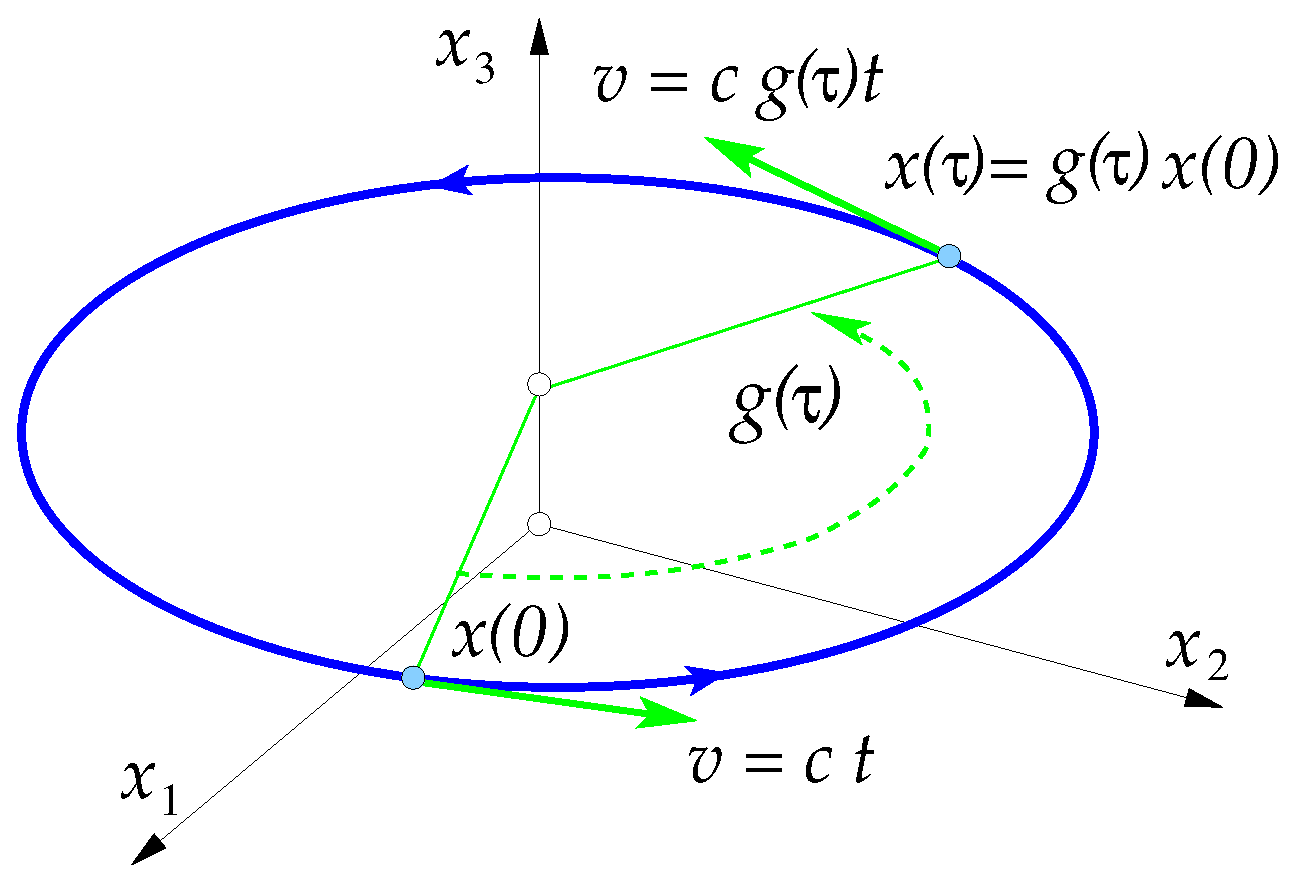
\includegraphics[width=0.3\textwidth]{../Fig/reqv.eps}
(b)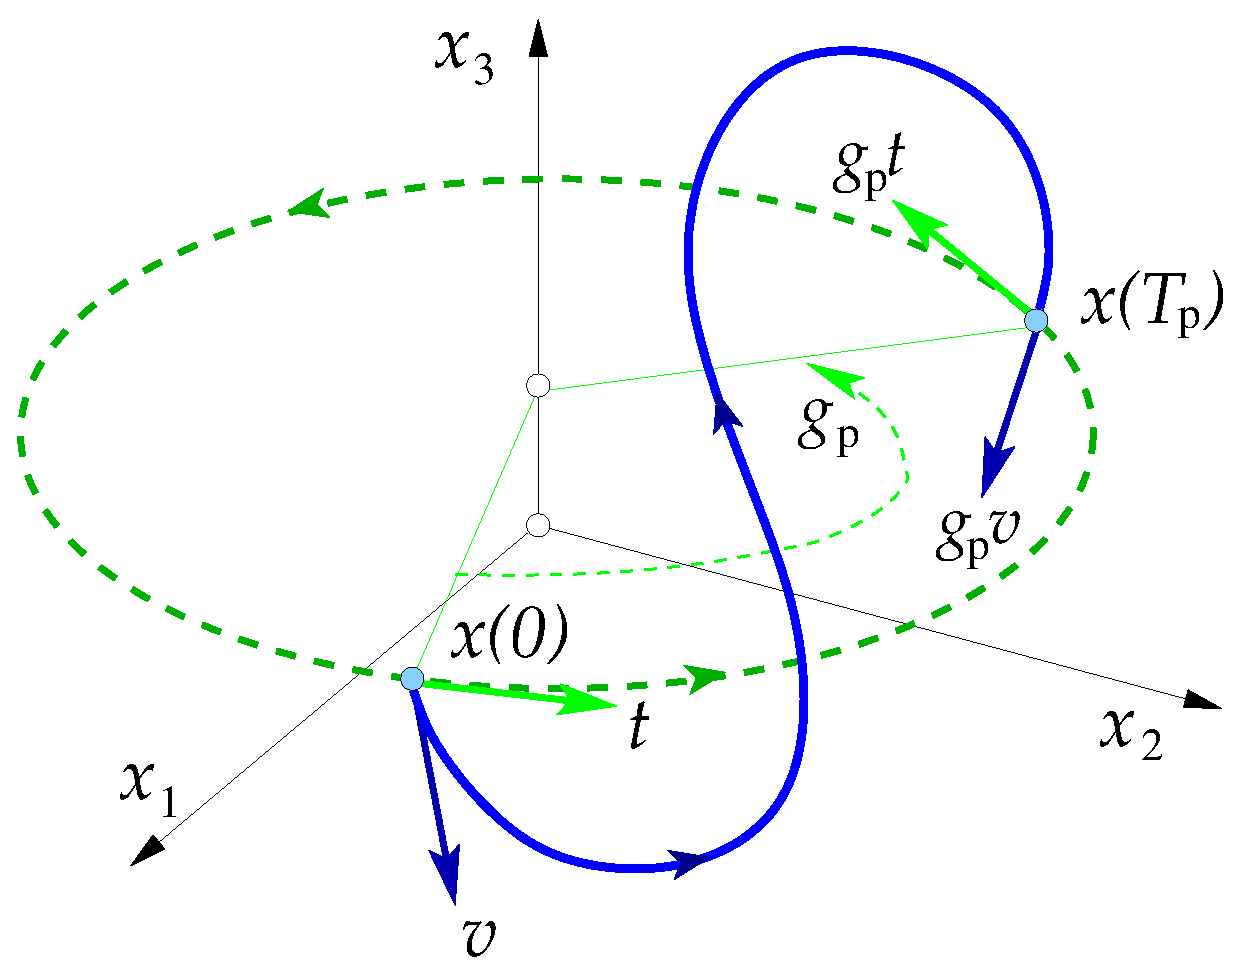
\includegraphics[width=0.3\textwidth]{../Fig/rpo.eps}
\caption{
(a) A {\em \reqv\ orbit} starts out at some point $\ssp(0)$,
with the dynamical flow field $\vel(\ssp) = \velRel \cdot
\groupTan(\ssp)$ pointing along the group tangent space. For
the $\SOn{2}$ symmetry depicted here, the flow traces out the
group orbit of $\ssp(0)$ in time $\period{}=2\pi/\velRel$.
An
{\em \eqv} lives either in the fixed $\Fix{\Group}$ subspace
($x_3$ axis in this sketch), or on a group orbit as the one
depicted here, but with zero angular velocity $\velRel$. In
that case the circle (in general, $N$-torus) depicts a
continuous family of fixed \eqva, related only by the group
action.
(b) A \rpo\ starts out at $\ssp(0)$ with the dynamical $\vel$ and
group tangent $\groupTan$ flows pointing in different
directions, and returns to the group orbit of $\ssp(0)$ after
time $\period{p}$ at $\ssp(\period{p})=\LieEl_p \ssp (0)$, a
rotation of the initial point by $\LieEl_p$.
}
\label{f:rpo}
\end{figure}
%%%%%%%%%%%%%%%%%%%%%%%%%%%%%%%%%%%%%%%%%%%%%%%%%%%%%%%%%%%%%%%%%%

Similarly to a \reqv, a \emph{\rpo} is periodic in its
mean velocity $\velRel_p=\gSpace_p/\period{p}$ co-rotating
frame (see \reffig{f:MeanVelocityFrame}), but in the
stationary frame its trajectory is quasiperiodic.
A co-moving
frame is helpful in visualizing a single `relative' orbit,
but useless for viewing collections of orbits, as each one
drifts with its own angular velocity. Visualization of all
\rpo s as \po s we attain only by global\marginpar{explain global vs
local in intro. It is not really global.} symmetry reduction,
to be undertaken in the following.

%
%%%%%%%%%%%%%%%%%%%%%%%%%%%%%%%%%%%%%%%%%%%%%%%%%%%%%%%%%%%%%%%%
% from siminos/rpo_ks/arxiv-v2/figs
\begin{figure}[ht]
(a)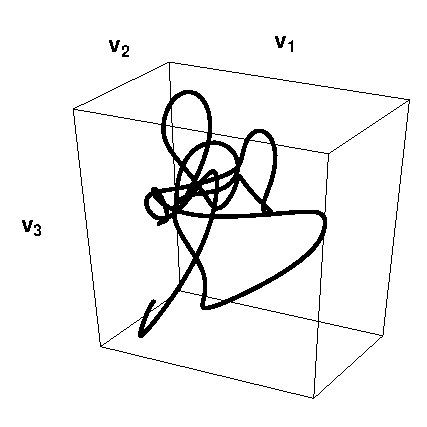
\includegraphics[width=0.37\textwidth, clip=true]
                    {../figs/ks22rpo033.50_04.045E2.eps}
~(b)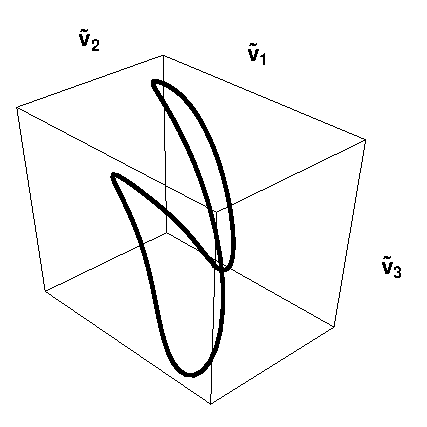
\includegraphics[width=0.37\textwidth, clip=true]
                     {../figs/ks22rpo033.50_04.045E2CM.eps}
\caption{
 A \rpo\ of Kuramoto-Sivashinsky flow projected on
 (a) the stationary \statesp\ coordinate frame
 $\{v_1,v_2,v_3\}$, traced for four periods
 $\period{p}$;
 (b) the co-moving $\{\tilde{v}_1,\tilde{v}_2,\tilde{v}_3\}$
 coordinate frame, moving with the mean angular velocity
 $\velRel_p=\gSpace_p/\period{p}$.
\hfill (from \refref{SCD07})
}
\label{f:MeanVelocityFrame}
\end{figure}
%%%%%%%%%%%%%%%%%%%%%%%%%%%%%%%%%%%%%%%%%%%%%%%%%%%%%%%%%%%%%%%%%%


